\subsection{Notary Scheme}
\label{sec:notary}
\subsubsection{Ripple Interledger protocol}
\noindent Earlier we focused on cross-chain, this project is more focused on cross-ledger, which means that the agreement not only supports decentralized blockchains but also supports various centralized ledgers, which is broader support for cross-chain applications. Ripple ILP\cite{thomas2015protocol} uses the HTLA and Notary scheme to implement this technology.\\
\noindent Ripple is the first project to propose the use of blockchain technology to achieve cross-ledger exchange of assets, with a focus on resolving cross-border remittances, enabling faster and more economical international remittances via the Ripple network.\\
\noindent Interledger Protocol(ILP) is compatible with any online ledger systems. Specifically, the ILP will establish a two-way pegged relationship between the trader's account and a Ripple local account, enabling simultaneous changes between the two to ensure transparency in the transaction process. At the same time, for two ledger systems that do not have a direct payment channel, multi-hop indirect cross-ledger transactions can be realized through ILP. \\
\noindent The main idea of ILP is to secure cross-ledger transactions by setting up \textit{escrow account} on Ripple. So the process will need the preparation of escrow account of several parties in the transaction. As an example in Figure \ref{fig:ILP}, Alice, Bob, and one selected market maker should have their own Ripple escrow accounts set up on two bank systems before the transaction. \\
\begin{itemize}
    \item Alice first selects a market maker with the most suitable exchange rate, and fill in the remittance information, receipt address and timeout period on the Ripple application.
    \item This information will be packed by the Interledger Module and sent to the Ripple Account 1, Ripple Account 1 records the changed amount of currency in the escrow account 1 and sends the transfer certificate to the \textbf{Validator}
    \item For Bob, Company B fills in the Ripple application with information such as the remittance address and timeout period and broadcasts it on the Ripple network. At this time, the liquidity provider selected by A will transfer a certain amount of assets in B's currency from Ripple Acc.3 to Ripple Acc.2 in advance, then send the transfer certificate to the \textbf{Validator}
    \item Validator checks the two transfer certificates; after the verification is passed, the ILP ledger will be liquidated simultaneously according to the Hashed Time Lock Agreement.
    \item The final step is when liquidation completed, Ripple will synchronize all account changes through an interledger module, thus realizing the cross-ledger transactions.
\end{itemize}
        \begin{figure}[H]
        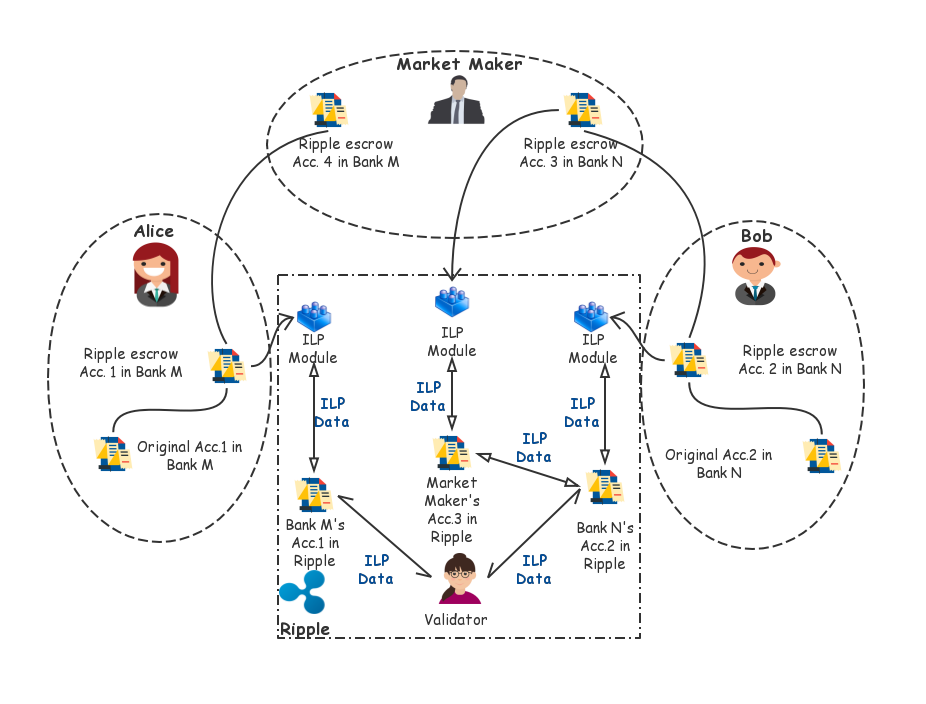
\includegraphics[width=1\textwidth]{./figures/ILP.png}
        \centering
        \caption{ILP example process}%\protect\footnotemark}
        \centering
        \label{fig:ILP}
        \end{figure}
        
\subsubsection{Liquid}
\noindent Liquid\cite{Liquid} is a sidechain of BTC and a typical representative of the multi-signature notary mechanism. It is designed to meet the BTC fast transfer needs of exchanges, market makers and brokers. Therefore, Liquid uses the multi-sig federation mechanism to confirm the transaction block, which can greatly improve the transaction speed.\\
\noindent Liquid based on Element codebase and uses Strong Federation technology to support 1:1 Bitcoin exchange. The basic process of the transaction is described as Figure \ref{fig:multisig}. The confirmation of this asset transfer requires multi-signature from the majority of notaries.

        \begin{figure}[H]
        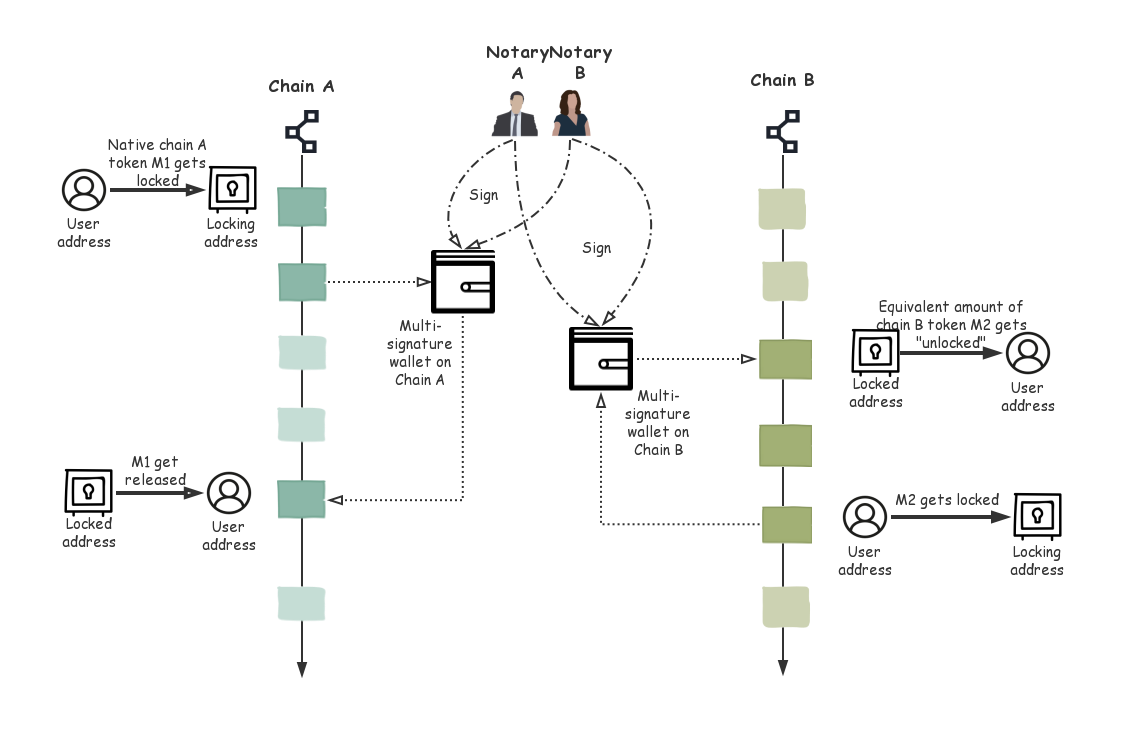
\includegraphics[width=1\textwidth]{./figures/multi_sig.png}
        \centering
        \caption{Multi-signature federation scheme}%\protect\footnotemark}
        \centering
        \label{fig:multisig}
        \end{figure}
        
\noindent In Strong Federation, there are 2 types of node role in the network:
\begin{itemize}
    \item Blocksigners: Signature verification for transactions in the sidechain to achieve block consensus. 
    \item Watchmen: When the asset is transferred from the sidechain to the main chain, it is responsible for signature verification of the transaction on the main chain, indicating that the sidechain asset has indeed been destroyed, and the main chain can unlock the corresponding number of assets.
\end{itemize}

\subsubsection{Wanchain}
\noindent Wanchain\cite{wanchain.org} is a cross-chain platform project initiated in 2016. It is a heterogeneous cross-chain framework that implements cross-chaining based primarily on distributed notary scheme. This model mainly uses cryptography "Secure Multi-Party Computation" and "Threshold Key Sharing Scheme" to implement the Authenticator distributed signature.\\

\noindent Wanchain provides the infrastructure for asset cross-chain transfer channels for different blockchain networks, realizing the transfer of assets between Wanchain and original chain. Wanchain3.0 now launches bridges from Bitcoin to the Ethereum network. The transaction reliability verification is completed by multiple Storeman of Wanchain. The following figures\ref{fig:wan1}\ref{fig:wan2} are shown the transfer process between Wanchain and Ethereum.
        \begin{figure}[H]
        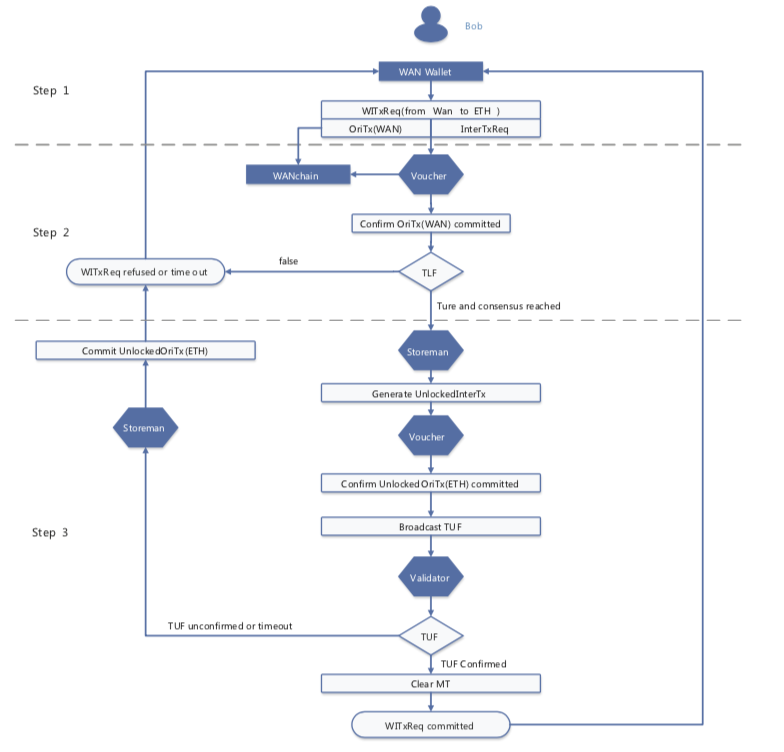
\includegraphics[width=1\textwidth]{./figures/ethtowan.png}
        \centering
        \caption{{Data transfer process from Ethereum to Wanchain}\protect\footnotemark}
        \centering
        \label{fig:wan1}
        
        \end{figure}
\footnotetext{Image courtesy of Wanchain white paper\cite{wanchain.org}}
        \begin{figure}[H]
        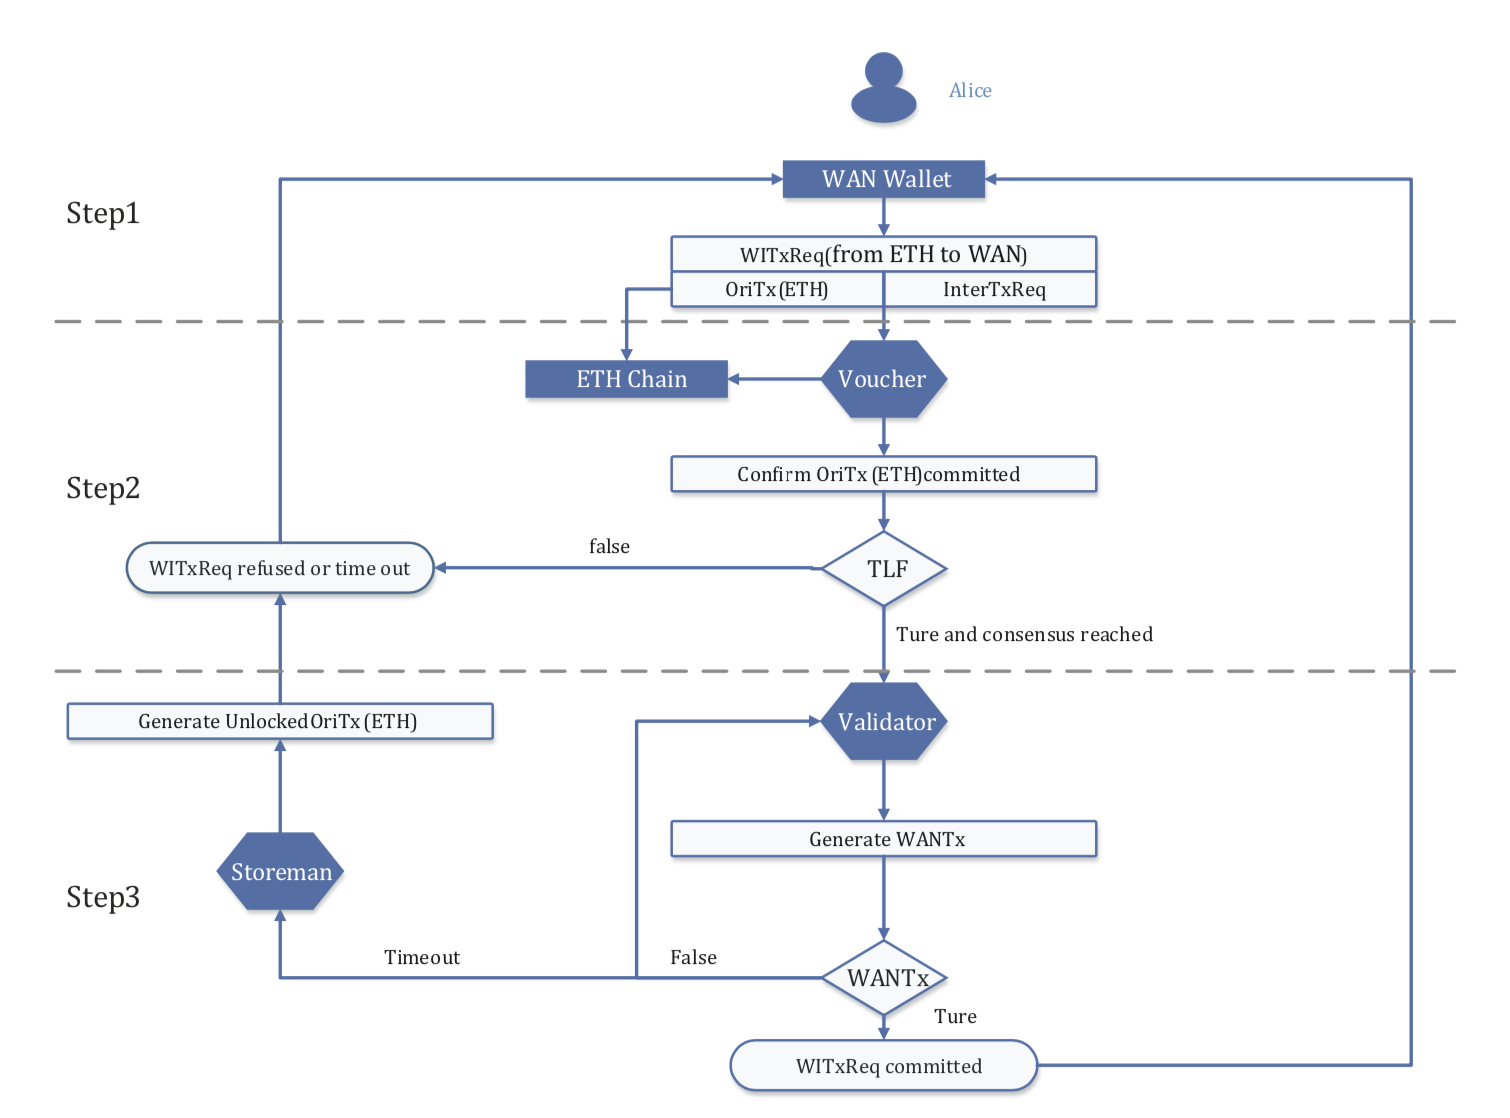
\includegraphics[width=1\textwidth]{./figures/wantoeth.png}
        \centering
        \caption{{Data transfer process from Wanchain to Ethereum}\protect\footnotemark}
        \centering
        \label{fig:wan2}
        
        \end{figure}
\footnotetext{Image courtesy of Wanchain white paper\cite{wanchain.org}}

\begin{enumerate}
    \item The token of the user in the original chain will be sent to Wanchain in the locked account, and the transaction is locked by Hash Time Lock;
    \item After the \textbf{Voucher} verified  the transaction on the original chain, the \textbf{Storeman} will initiate a cross-chain contract transaction on the Wanchain, and transfer the mapping token in wanchain to the user's cross-chain account on Wanchain, and locked;
    \item After the user's wallet detects the transaction locked by the cross-chain contract, release the Secret to the cross-chain contract;
    \item Storeman obtains the control of the original chain token through the secret number, thus achieving confirmation of the original chain transaction.
    \item If the user does not release the secret number within the scope of the hash time lock, the hash time lock expires
    \item The transaction of the post-cross-contract is automatically invalidated, and the user regains control of the original token.
\end{enumerate}

\noindent In Wanchain, when Storeman locked an account, the private key of the locked account is scattered into multiple pieces and send to Storeman, and it requires more than a certain percentage of Storeman complete the signature before the final confirmation. In order to avoid conspiracy, Storeman has to pay a certain amount of token to participate in the verification in case of doing evil. To ensure atomicity, Wanchain uses a hash time lock to lock cross-chain transactions, ensuring that no user or Storeman will complete a one-sided transaction.\\

\noindent Since the Wanchain mechanism does not change the original chain, it is necessary to adapt the development according to the characteristics of the original chain, which is also the difficulty of heterogeneous cross-chain solution. The transaction speed is affected by the confirmation speed of the original chain.\\\\
\begin{large}
\textbf{Fusion}
\end{large}\cite{fusion}\\


\noindent Similar to the principle of Wanchain, Fusion's goal is to build a basic platform for the operation of encrypted financial applications based on blockchain technology. On this platform, a variety of tokens can be freely interacted through smart contracts to achieve value interoperability. Support multi-platform cross-chain asset transfer, using a distributed signature notary model for cross-chain transaction processing.\\

\noindent Based on Hierarchical Hybrid Consensus Mechanism(HHCM), Fusion combines the advantages of PoW and PoS consensus mechanism, which balancing the safety, efficiency, and scalability. It is the only cross-chain platform that offers parallel computing, multiple triggering mechanisms, and off-chain data support.\\

        \begin{figure}[H]
        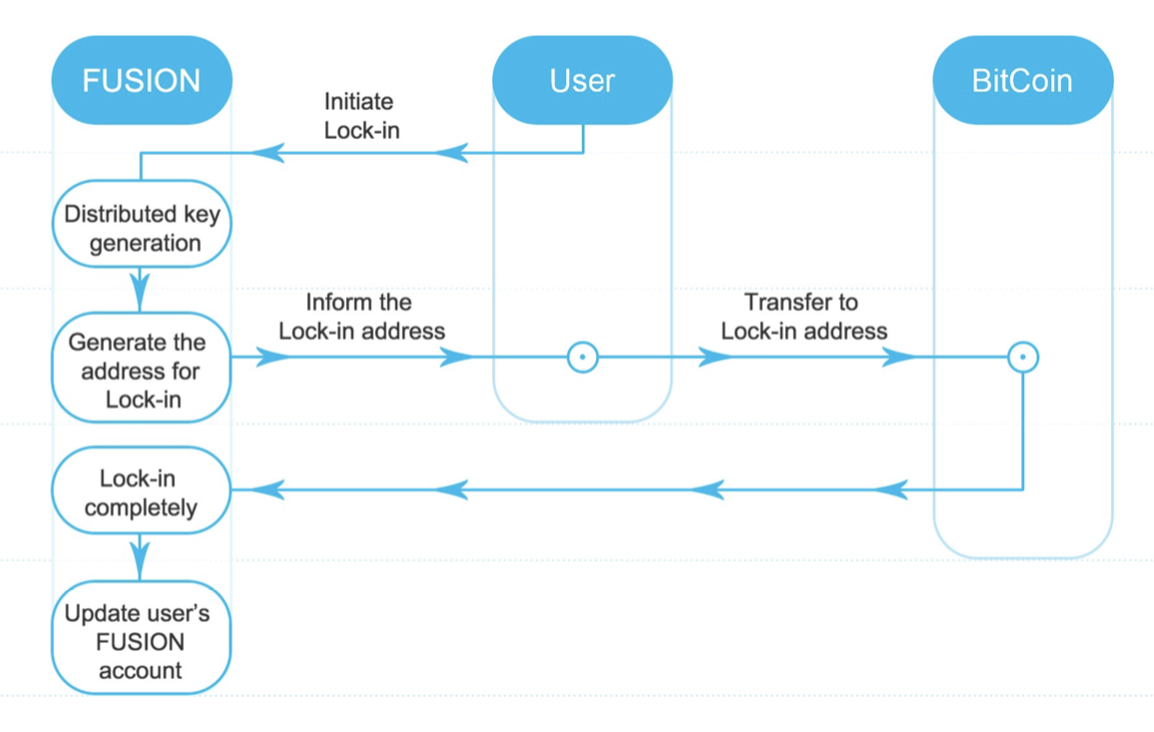
\includegraphics[width=1\textwidth]{./figures/lockin}
        \centering
        \caption{{Fusion Network Architecture, lock-in process}\protect\footnotemark}
        \centering
        \label{fig:lockin}
        
        \end{figure}
\footnotetext{Image courtesy of Fusion white paper\cite{fusion}}
\noindent The realization of cross-chain assets transaction is based on the lock-in\&lock-out process as shown in Figure \ref{fig:lockin}.
